<<echo=FALSE, cache=FALSE>>=
set_parent('./project.Rnw')
@
%%fakesection Boosting
In this chapter two boosting algorithms will be discussed, \textit{Adaboost} and \textit{Gradient Boosting}. First the basic framework will be introduced, much through Adaboost, but the main focus will be on Gradient Boosting based on trees. 

Boosting algorithms combine many ''weak'' classifiers to create one ''strong'', and goes under the class of committee-based classifiers. The weak classifiers are usually high biased with low variance, so boosting is often referred to as a bias reducing method. 

The algorithms train weak classifiers sequentially, and for each new classifier the data points are weighted by how hard they were for previous classifiers to classify correctly. At the end all the classifiers are combined and weighted based on how well they perform. The idea is better illustrated in the \textit{Adaboost.M1} algorithm by  \cite{adaboostM1}.
\section{Adaboost}
\label{sec:Adaboost}
Adaboost is perhaps the most historically significant boosting algorithm and Adaboost.M1 is one of its most basic versions. \cite{modstat} described it as ''the most popular boosting algorithm'', and \cite{Breiman1996} as ''the best of-the-shelf classifier in the world''. Adaboost.M1 only considers two classes, but it generalizes easily to multiple classes through Adaboost.M2 \citep{adaboostM1}. 

An important restriction on both methods is that the weak classifiers are required to have prediction error less than $0.5$.
Consider the output variable coded as $y \in \{-1, 1\}$. A weak classifier $C_m(\mathbf{x})$ is chosen to do the ground work. This can for instance be a shallow tree, or some other algorithm that does not perform much better than random guessing. All the data points $\mathbf{x}_i$, $i = 1, 2, \ldots, N$, are initialized with weights $w_i = 1/N$. Then, for $m = 1, \ldots, M$, $C_m(\mathbf{x})$ is trained using $w_i$. $err_m$ is used as a performance measure for $C_m(\mathbf{x})$,
\begin{align}
  err_m =  \frac{\sum^{N}_{i=1} w_i I\{y_i \neq C_m(\mathbf{x}_i)\}}{\sum^{N}_{i=1} w_i}.
\end{align}
The weights are updated using, 
\begin{align}
  w_i &\leftarrow w_i \exp\left( \alpha_m I\{y_i \neq C_m(\mathbf{x}_i)\} \right), \\
  &\text{where} \quad \alpha_m = \log\left(  \frac{1-err_m}{err_m} \right).
\end{align}
Finally the classifier is created,
\begin{align}
  C( \mathbf{x}) = \text{sign}\left( \sum^{M}_{m=1} \alpha_m C_m(\mathbf{x}) \right).
\end{align}
There are many choices of weak classifiers, but one of the more common is to use classification trees. In that case it is important to not grow an optimal tree as with CART, but instead grow a shallow tree or just stumps (one split). The size of the individual trees will be discussed in Section~\ref{sub:Tree size}. For computational purposes, the trees are only grown and not pruned back.
An example of this implementation can be found in the R package \verb+adabag+ by \cite{adabag}, that use the \verb+rpart+ implementation of CART by \cite{rpart} as base classifiers.

\section{Forward stagewise additive modeling}
\label{sec:Forward stagewise additive modeling}
A common way to view the goal of classification problems is through the expected prediction error discussed in Section~\ref{sub:LDA}. The goal is to find,
\begin{align}
  \label{eq:fargmin} 
  f^* = \argmin_f \E_{y, \mathbf{x}}[L(y,f(\mathbf{x}))] = \argmin_f \E_y [L(y,f(\mathbf{x})) \mid \mathbf{x}\:] ,
\end{align}
where $L(y, f(\mathbf{x}))$ is some loss function. 
Note that $L$ does not necessarily need to be the misclassification rate, even though the actual objective is to minimize it.
Often it is hard to work with, as it is not continuous, and a continuous approximation is used as a substitute.

Even with continuous loss, $f^*$ is often hard to obtain. A common procedure is to restrict $f$ to be a member of a parameterized class of functions. In this section $f$ will be an additive expansion in a set of elementary basis functions,
\begin{align}
  \label{eq:additive} 
  f(\mathbf{x}) =  \sum^{M}_{m=1} \beta_m h(\mathbf{x}; \bm{\gamma}_m).
\end{align}
Here $h$ is usually a simple function of $\mathbf{x}$ and parameters $\bm{\gamma}$. These expansions are common tools in classification and are used in techniques like Neural Networks, Wavelets, MARS and Support Vector Machines.

Under \eqref{eq:additive}, the solution of \eqref{eq:fargmin} is usually still hard to obtain. Therefor \textit{forward stagewise additive modelling} approximates the solution by sequentially adding new basis functions without changing parameters of basis functions already fitted. The algorithm works the following way:\\
\\
$f_0$ is initialized to 0. For $m = 1, \ldots, M$, $\beta_m$ and $\bm \gamma_m$ is found by
\begin{align}
  \label{eq:forStageWise} 
  (\beta_m, \bm \gamma_m) = \argmin_{\beta, \bm \gamma} \sum^{N}_{i=1} L(y_i, f_{m-1}(\mathbf{x}_i) + \beta h(\mathbf{x}_i; \bm \gamma)).
\end{align}
$f_m(\mathbf{x})$ is updated by $f_m(\mathbf{x}) = f_{m-1}(\mathbf{x}) + \beta_m h(\mathbf{x}; \bm \gamma_m)$.\\
\\
If the basis functions are set to be a classifier $h(\mathbf{x}; \bm \gamma) \in \{-1, 1\}$, and the loss is exponential,
\begin{align}
  \label{eq:expLoss} 
  L(y, f(\mathbf{x})) = \exp (-y f(\mathbf{x})),
\end{align}
it can be shown [\cite{modstat}] that forward stagewise additive modeling is equivalent to the Adaboost.M1 classifier. However, this was not the original motivation for Adaboost.M1. The way Adaboost.M1 fits in the forward stagewise framework, was only discovered years later. Nevertheless, the forward stargewise framework provides opportunity to further study Adaboost.M1, and compare it to other loss functions. Under the exponential loss in \eqref{eq:expLoss}, the solution to \eqref{eq:fargmin} is,
\begin{align}
  f^*( \mathbf{x}) = \frac{1}{2} \log \frac{P(y=1 \mid \mathbf{x})}{P(y=-1 \mid \mathbf{x})} .
\end{align}
So the classification rule in Adabost.M1 approximates one half of the log-odds. This justifies using its sign as a classification rule.
%
\subsection{Loss functions}
\label{sub:Loss functions}
<<lossFunctions, echo=FALSE>>=
# Plot of different loss functions
source("../code/lossFunctions.R")
@
The choice of loss function is important in terms of both accuracy and computational cost. While the use of $0/1$ loss might be intuitive, a differentiable loss function might give a computational advantage. By using squared error loss, $L = (y - f(\mathbf{x}))^2$, \eqref{eq:forStageWise} fit a basis function to the residual of the previous function. There exist fast algorithms for solving these type of problems, but squared error loss is still not considered a good choice for classification. That can be explained by Figure~\ref{fig:lossFunctions}. The figure shows the loss $L(y, f(\mathbf{x}))$ for different loss functions, where $y \in \left\{ -1, 1 \right\}$. If the classification rule is $C(\mathbf{x}) = \mathrm{sign}(f(\mathbf{x}))$, then a positive margin $y f(\mathbf{x}) > 0$ implies a correct classification, while a negative margin implies a wrong. It is clear from the figure that squared error loss start increasing when the margin is higher than $1$. As loss functions should penalize a negative margin more than a positive, squared error loss is unsuited for classification.
%
\begin{figure}[htbp]
\begin{center}
    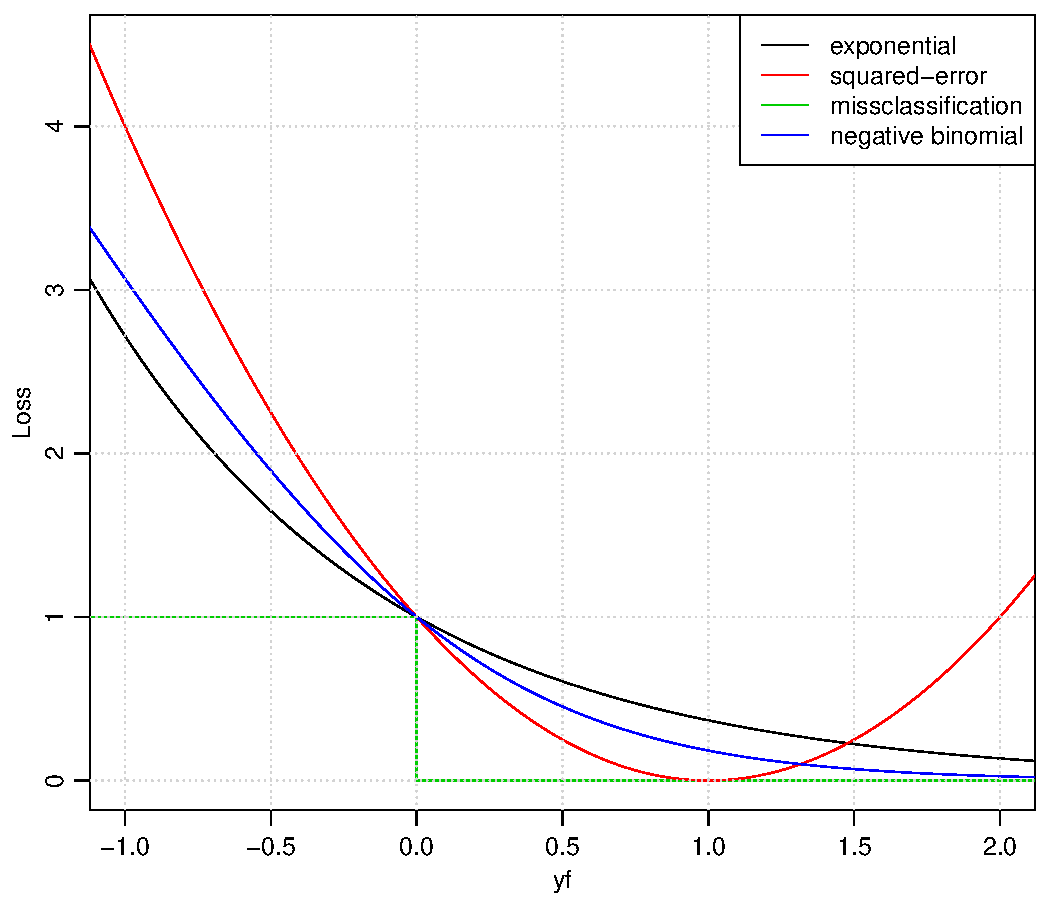
\includegraphics[scale=0.5]{./figures/lossFunctions.pdf}
\end{center}
\caption{Different loss functions $L(y, f)$ as function of the margin $yf$, scaled so all goes through point $(0, 1)$. $y \in \{-1, 1\}$.}
\label{fig:lossFunctions}
\end{figure}
%

From the figure it is clear that exponential and misclassification loss decrease with the margin and are therefore better choices than squared error loss. But as mentioned earlier, and will become more clear in Section~\ref{sec:Gradient Boosting}, a differentiable loss gives some computational advantages. The last loss function in Figure~\ref{fig:lossFunctions} is the \textit{negative binomial log-likelihood}, or \textit{binomial deviance},
\begin{align}
  L(y, f(\mathbf{x})) = \log \left( 1 + \exp (-2 y f(\mathbf{x})) \right).
\end{align}
It is very similar to the exponential loss. The main difference is that for increasingly negative margins the exponential loss penalize exponentially, while the binomial deviance penalize linearly. Therefore the binomial deviance is not as vulnerable in noisy settings. The binomial deviance is a very common choice and will be the main focus for the rest of this chapter. 
\\
\\
For multiclass cases, the binomial deviance generalizes to the \textit{multinomial deviance},
\begin{align}
  \label{eq:multinomialDeviance} 
  &L(y, \mathbf{f}( \mathbf{x })) = - \sum^{K}_{k=1} I\{y = k\} \log p_k(\mathbf{x}), \\
  \label{eq:multinomialDevianceProb} 
  &\text{where} \quad p_k(\mathbf{x}) = \frac{\exp (f_k(\mathbf{x}))}{\sum^{K}_{l=1} \exp (f_l(\mathbf{x}))}\\
  &\text{and} \quad \mathbf{f} = (f_1, \ldots, f_K)^T.
\end{align}
A generalization of the exponential loss for multiple classes can be found in \cite{zhu2009}.
\section{Gradient Boosting}
\label{sec:Gradient Boosting}
%%fakesubsection Gradient Boosting
Gradient Boosting is a method developed by \cite{friedman}. It is built on the forward stagewise framework for arbitrary differentiable loss functions, and the idea is to solve for $f^*$ in \eqref{eq:fargmin} numerically, using steepest decent in function space.

Let $g_m$ denote the gradient at step $m$,
\begin{align}
  g_{m}(\mathbf{x}) = \left[ \frac{\partial \E_{y} [ L(y, f(\mathbf{x})) \mid \mathbf{x}\:]}{\partial f(\mathbf{x})}  \right]_{f(\mathbf{x}) = f_{m-1}(\mathbf{x})},
\end{align}
or, assuming sufficient regularity that integration and differentiation can be interchanged, 
\begin{align}
  g_{m}(\mathbf{x}) = \E_{y} \left[ \frac{\partial L(y, f(\mathbf{x})) }{\partial f(\mathbf{x})}  \mid \mathbf{x}\right]_{f(\mathbf{x}) = f_{m-1}(\mathbf{x})}.
\end{align}
$f_m$ is updated by,
\begin{align}
  f_m(\mathbf{x}) = f_{m-1}(\mathbf{x}) - \rho_m  g_m(\mathbf{x}),
\end{align}
where $\rho_m$ is the step length found by,
\begin{align}
  \rho_m = \argmin_{\rho}  \E_{y} [ L(y, f_{m-1}(\mathbf{x}) - \rho g_m(\mathbf{x}))  \mid \mathbf{x}\:].
\end{align}
By repeating these steps, the function is moving towards a minimum of $L$ (in the steepest decent direction $-g_m$), though in a very greedy matter. 

In the steepest decent algorithm above $\mathbf{x}$ and $y$ are considered a stochastic variables, but in practice their distributions are not known. For finite data $\{\mathbf{x}_i, y_i\}_{i = 1}^{N}$, $E_y \left[\: \cdot \mid \mathbf{x} \right]$ can not be accurately estimated, and $g_m(\mathbf{x})$ is defined only at the data points. As the goal is to find a good approximation for $f^*(\mathbf{x})$ for all $\mathbf{x}$, a different approach is needed. 
\\
\\
Impose a parameterized form of $f$ in the form of additive basis functions, and return to the forward stagewise additive modeling problem in \eqref{eq:forStageWise}. Suppose this problem is hard to solve under the constraints of the basis functions $h(\mathbf{x}; \bm \gamma)$.
In this framework, for a given $f_{m-1}(\mathbf{x})$, the function $\beta_m h(\mathbf{x}; \bm{\gamma}_m)$ can be viewed as the best greedy step toward the training based $f^*$, under the constraint of the parameterization. It can thus be considered a steepest decent step, and $\mathbf{h}_m = [h(\mathbf{x}_1; \bm\gamma_m), \ldots, h(\mathbf{x}_N; \bm\gamma_m)]^T$ is comparable to the data based unconstrained negative gradient $-\mathbf{g}_m = [-g_m(\mathbf{x}_1), \ldots, -g_m(\mathbf{x}_N)]^T$, where,
\begin{align}
  -g_{m}(\mathbf{x}_i) = -\left[ \frac{\partial L(y_i, f(\mathbf{x}_i)) }{\partial f(\mathbf{x}_i)} \right]_{f(\mathbf{x}) = f_{m-1}(\mathbf{x})}.
\end{align}
So $ \mathbf{h}_m$ can instead be fitted to $-\mathbf{g}_m$. This is done by finding the $h(\mathbf{x}; \bm{\gamma}_m)$ highest correlated to $-g_m(\mathbf{x})$,
\begin{align}
  \label{eq:gradBoostFit} 
  \bm \gamma_m = \argmin_{\beta, \bm \gamma} \sum^{N}_{i=1} \left( -g_m(\mathbf{x}_i) - \beta h(\mathbf{x}_i; \bm \gamma) \right)^2.
\end{align}
Then $f_m$ is updated using,
\begin{align}
  &f_m(\mathbf{x}) = f_{m-1}(\mathbf{x}) + \rho_m h(\mathbf{x}; \bm{\gamma}_{m}),\\
  \label{eq:lineSearch} 
  &\text{where} \quad \rho_m = \argmin_\rho \sum^{N}_{i=1} L(y_i, f_{m-1}(\mathbf{x}_i) + \rho h(\mathbf{x}_i; \bm{\gamma}_m)).
\end{align}
These last three equations are know as the \textit{Gradient Boosting} algorithm.
As \eqref{eq:forStageWise} is replaced by \eqref{eq:gradBoostFit} and \eqref{eq:lineSearch}, $\tilde{y}_i = -g_m(\mathbf{x}_i)$ is often referred to as the ''pseudo-response''. 

Note here that $h$ and $f$ are continuous functions and not classifiers. The classification is done after all the $M$ iterations, usually trough some relationship between $f_M$ and class probabilities. For the binomial deviance loss this relationships are the log-odds,
\begin{align}
  \label{eq:boostLogOdds1} 
  &\hat P(y = 1 \mid  \mathbf{x}) = \left( 1+ \exp\left( -2 f_M (\mathbf{x}) \right) \right)^{-1},\\
  \label{eq:boostLogOdds2} 
  &\hat P(y = -1 \mid \mathbf{x}) = \left( 1+ \exp\left( 2 f_M (\mathbf{x}) \right) \right)^{-1}.
\end{align}
\subsection{Regression Trees}
\label{sub:Regression Trees}
It was earlier mentioned that the basis functions $h(\mathbf{x}; \bm{\gamma}_m)$ in Gradient Boosting need to be able to approximates continuous functions. Therefore, classification trees can not be used and the regression framework needs to be explored.
Section~\ref{sec:CART} showed how classification trees can be fitted using the CART method. CART stands for \textit{Classification And Regression Trees} and can obviously also be used for regression. The procedure for fitting of regression trees is almost identical to that for classification, but the functions used during growing and pruning are different. However, this will not be investigated deeply. This section discuss only how trees can be used in the boosting framework.\\
\\
A regression tree $T$ can be represented on the following form,
\begin{align}
  T(\mathbf{x}; \left\{ c_j, R_j \right\}_{j = 1}^J)  = \sum^{J}_{j=1} c_j I\left\{ \mathbf{x} \in R_j \right\}.
\end{align}
As with classification all the regions $R_j$ are disjunct and collectively cover all possible values of $\mathbf{x}$. 
When fitting a tree to the response $\tilde y$ under squared error loss, it is straight forward to see that the solution in each region $R_j$ is just the region average,
\begin{align}
  \hat{c}_j = \mathrm{ave}\{\tilde y_i \mid \mathbf{x}_i \in R_j\}.
\end{align}
The tree is grown sequentially, by finding the split that minimize the total squared error loss. When a larger tree is grown, it can then be pruned back using \textit{cost-complexity pruning} based on the squared error and penalized by the number of terminal nodes. In the boosting context however, pruning is not really an alternative. According to \cite{modstat}, usually $J \leq 10$ end-nodes will be sufficient, and thus growing a larger tree and pruning it back will only be very costly without much effect on the end results. The tree size will be further discussed in Section~\ref{sub:Tree size}.\\
\\
In Gradient Boosting, trees are fitted in \eqref{eq:gradBoostFit}, in place of $\beta h(\mathbf{x}_i; \bm{\gamma})$. Thus $f_m$ is given by, 
\begin{align}
  f_m(\mathbf{x}) = f_{m-1}(\mathbf{x}) + \rho_m T(\mathbf{x}; \left\{ c_{m j}, R_{m j} \right\}_{j=1}^{J}),
\end{align}
where $\rho_m$ is the solution of the line search in \eqref{eq:lineSearch}.  However, it is more common to use \textit{one} variable $\eta_{m j}$ instead of $\rho_m c_{m j}$. 
As the trees are disjunct, each $\eta_{m j}$ can be found independently.
This way $J$ separate basis functions are fitted instead of one single additive, giving better opportunity to tune the coefficients. So $f_m$ is set to,
\begin{align}
  &f_m(\mathbf{x}) = f_{m-1}(\mathbf{x}) +  \sum^{J}_{j=0} \eta_{m j} I\left\{ \mathbf{x} \in R_{m j} \right\}, \\
  \label{eq:etaLineSearch} 
  &\text{where} \quad
  \eta_{m j} = \argmin_\eta  \sum_{\mathbf{x}_i \in R_{m j}} L(y_i, f_{m-1}(\mathbf{x}_i) + \eta).
\end{align}

\subsection{The two-class logistic regression classifier}
\label{sub:The two-class logistic regression classifier}
The framework for Gradient Boosting is now reviewed, and as a final step the algorithm is summarize under binomial deviance loss. As before $y \in \left\{ -1, 1 \right\}$ and the loss is,
\begin{align}
  &L(y, f(\mathbf{x})) = \log (1 + \exp (-2 y f(\mathbf{x}))),\\
  &\text{where} \quad f(\mathbf{x}) = \frac{1}{2} \log \frac{ P(y = 1 \mid \mathbf{x})}{ P(y = -1 \mid \mathbf{x})}  .
\end{align}
$f_0(\mathbf{x})$ is initialized to $\frac{1}{2} \log \frac{1+\bar{y}}{1-\bar{y}}$.  The pseudo-response is,
\begin{align}
  \label{eq:ytildeGradboost} 
  &\tilde{y}_i = 
  -\left[ \frac{\partial L(y_i, f(\mathbf{x}_i)) }{\partial f(\mathbf{x}_i)}  \right]_{f(\mathbf{x}) = f_{m-1}(\mathbf{x})}
  = 2 y_i / (1 + \exp \left( 2 y_i f_{m-1}(\mathbf{x}_i) \right), \quad i = 1, \ldots, N.
\end{align}
A regression tree $T$ is fitted to the $\tilde y_i$'s,
\begin{align}
  \left\{ R_{m j} \right\}_{j = 1}^J  = 
  \argmin_{\left\{ c_j, R_{j} \right\}_{j = 1}^J} \sum^{N}_{i=1} \left( \tilde y_i - T(\mathbf{x}_i; \left\{ c_j, R_j \right\}_{j = 1}^J) \right)^2.
\end{align}
The line searches in \eqref{eq:etaLineSearch} become,
\begin{align}
  \eta_{m j} = \argmin_\eta  \sum_{\mathbf{x}_i \in R_{m j}} \log (1 + \exp [-2 y_i (f_{m-1}(\mathbf{x}_i) + \eta) ]), \quad j = 1, \ldots, J.
\end{align}
These optimization problems have no closed form solution. A common way to approximate the solution is by doing a Newton-Raphson step instead,
\begin{align}
  \eta_{m j} =  \frac{\sum_{\mathbf{x}_i \in R_{m j}} \tilde y_i}{\sum_{\mathbf{x}_i \in R_{m j}} |\tilde y_i|(2-|\tilde y_i|)}.
\end{align}
Here  $\tilde y_i$ is the pseudo response in \eqref{eq:ytildeGradboost}. $f$ can now be updated by,
\begin{align}
  \label{eq:gradBoostUpdateF} 
  f_m(\mathbf{x}) = f_{m-1}(\mathbf{x}) +  \sum^{J}_{j=0} \eta_{m j} I\left\{ \mathbf{x} \in R_{m j} \right\}.
\end{align}
All this is repeated $M$ times, and classification can be done based on the log odds, as mentioned in \eqref{eq:boostLogOdds1} and \eqref{eq:boostLogOdds2}. \\
\\
It is not hard to generalize the algorithm to the multiple classes. As mentioned earlier, the binomial deviance generalizes to the multinomial deviance in \eqref{eq:multinomialDeviance}. As there are now $K$ functions $f_k$, $K$ different trees has to be fitted at each iteration, one for each pair $(\tilde y_{k i}, f_k)$. Correspondingly, $J$ coefficients $\eta_{m k j}$ has to be fit for each tree, using the Newton-Raphson step. At the end the classifier is created based on the estimated class probabilities in \eqref{eq:multinomialDevianceProb}. For more details see \cite{friedman}.

\section{Tuning boosting algorithms}
\label{sec:Tuning boosting algorithms}
Boosting algorithms have parameters that need to be set by the user. These can have a great impact on both performance and time, and often depend on each other. The first parameter that might come to mind is the number of boosting iterations $M$. It controls much of the balance between underfitting and overfitting. The choice for $M$ is usually made through either a test set, if there is a large amount of data, or through cross-validation. It is also possible to use the \textit{Out-of-bag} estimates for  \textit{Stochastic Gradient Boosting} (see Section~\ref{sec:Stochastic Gradient Boosting}). This will be discussed in Section~\ref{sub:Out-of-bag}.

\subsection{Tree size}
\label{sub:Tree size}
The number of terminal nodes $J$ in the trees control the bias-variance tradeoff in the individual classifiers, as discussed in Section~\ref{sec:Tree}.  Large trees have high variance and low bias, while small trees have the opposite.   Following the reasoning in \cite{modstat} and \cite{friedman}, the goal is to find $f^*$ solving \eqref{eq:fargmin}. Consider an ANOVA expansion of the solution,
\begin{align}
  \label{eq:ANOVAexpansion} 
  f^*(\mathbf{x}) = \sum_{i} f_i(x_i) + \sum_{ij} f_{ij}(x_i, x_j) + 
  \sum_{ijk} f_{ijk}(x_i, x_j, x_k) + \cdots,
\end{align}
where $\mathbf{x} = (x_1, x_2, \ldots, x_p)^T$. $f_i$ is called the \textit{main-effect}, $f_{ij}$ the \textit{second order interaction}, $f_{ijk}$ the \textit{third order interaction}, and so on. The expansion is such that the first sum is the best approximation to $f^*$ under the constraint of only main-effects. The second sum gives the best approximation to $f^*$ under the constrain of only main-effects and second order interactions. This way \eqref{eq:ANOVAexpansion} can be viewed as an additive model. 

When fitting an additive model of trees with only two terminal nodes (commonly referred to as stumps), these will have the same structure as the main-effects. To capture interactions of order up to $J$, a tree with $J+1$  terminal nodes is needed. However, by setting $J$ to large, unnecessary variance is introduced in the trees. Boosting methods works by lowering the bias through the forward stagewise process, so it might be advantageous to use high bias low variance trees, but ideally one would of course try to be close to the dominant interaction order of $f^*$.
According to \cite{modstat}, $4 \leq J \leq 8$ usually works well, and $J>10$ is rarely needed.  

\subsection{Shrinkage}
\label{sub:Shrinkage}
As previously discussed, regularization is mainly controlled by number of boosting iterations $M$. However, \cite{copas1983} shows that \textit{shrinkage} might improve the results compared with only restricting on $M$. For the Gradient Boosting algorithm it is straight forward to include this. 
The update of $f$ in \eqref{eq:gradBoostUpdateF} is just changed to,
\begin{align}
  f_m(\mathbf{x}) = f_{m-1}(\mathbf{x}) +  \nu \sum^{J}_{j=0} \eta_{m j} I\left\{ \mathbf{x} \in R_{m j} \right\}, \quad 0 < \nu < 1,
\end{align}
or more generally in the forward stagewise framework,
\begin{align}
  f_m(\mathbf{x}) = f_{m-1}(\mathbf{x}) +  \nu \: \beta_m h(\mathbf{x}; \bm \gamma_m), \quad 0 < \nu < 1.
\end{align}
Here $\nu$ is often referred to as the \textit{learning rate} or \textit{shrinkage parameter}. \cite{friedman} shows that empirically, smaller values of $\nu$ give better test error. However, it requires a correspondingly larger $M$. 


\subsection{Influence trimming}
\label{sub:Influence trimming}
Under binomial deviance loss, at the $m$'th iteration, the problem at hand is to minimize,
\begin{align}
  \label{eq:influence} 
  \sum_{i = 1}^{N} \log \left( 1 + \exp[ -2 y_i f_{m-1}(\mathbf{x}_i)] \exp [-2 y_i \rho h(\mathbf{x}_i; \bm \gamma)] \right),
\end{align}
over $\rho$ and $\bm \gamma$.  For $y_i f_{m-1}(\mathbf{x}_i)$ large, the effect of of $\rho h(\mathbf{x}_i; \bm{\gamma})$ is very small, and the minimization of \eqref{eq:influence} is more or less independent of $\rho h(\mathbf{x}_i; \bm \gamma)$. This means that the data point $(\mathbf{x}_i, y_i)$ can be removed from the calculations, without any substantial effect on $\rho$ and $\bm \gamma$. Removing such points during training is called \textit{influence trimming}, and can speed up the calculations. \cite{friedman} therefore proposed,
\begin{align}
  w_i = \exp (- 2 y_i f_{m-1}(\mathbf{x}_i)), 
\end{align}
as an measure for influence. 

More generally, the influence can be measured, by the second derivative of the loss function,
\begin{align}
  w_i = \left[ \frac{\partial^2 L(y_i, f(\mathbf{x}_i)) }{\partial f(\mathbf{x}_i)^2}  \right]_{f(\mathbf{x}) = f_{m-1}(\mathbf{x})}.
\end{align}
This is because the first derivative is close to zero for optimal values for $\rho$ and $\bm \gamma$, so the second derivative gives a more stable measure.  For the binomial loss, this becomes,
\begin{align}
  w_i = |\tilde y_i| \: (2 - |\tilde y_i|). 
\end{align}
Removing points with low influence can have a considerable impact on computing time, while leaving the estimates relatively untouched. 

\section{Stochastic Gradient Boosting}
\label{sec:Stochastic Gradient Boosting}
Bagging was introduced by \cite{Breiman1996} and will be covered in Section~\ref{sec:Bagging}. He showed that the performance of function estimation procedures could be improved by introducing randomness in the training data. 
Inspired by this, in addition to the randomization of Adaboost by \cite{freund1996} and the hybrid procedure of boosting and bagging by \cite{breiman1999}, \cite{FriedmanStochBoost} developed the \textit{Stochastic Gradient Boosting} algorithm.
This new method is only a slight modification of the Gradient Boosting algorithm, but has been shown capable of outperforming Gradient Boosting, both in terms of accuracy and computation time.  

The idea is, sample a subset of the training data, without replacement, at each iteration. All the steps are exactly the same as in the Gradient Boosting algorithm, but they are performed on the subset. \\
\\
The size of the subset, $N_{sub}$, introduce another tuning parameter. Smaller values of $N_{sub}$ introduce more randomness to the procedure, while reducing computing time by the fraction $N_{sub}/N$. However, as the data trained on at each iteration becomes smaller, the variance of the individual base learners will increase. The gain comes from reduction in the correlation between estimates at each iteration, as this tend to reduce the variance of the combined model \eqref{eq:additive}.

For $N_{sub} = 0.5$, the algorithm is approximately equivalent to drawing bootstrap samples. Therefore, \cite{modstat} propose that typical values for $N_{sub}$ should be around $0.5$, but can be made substantially lower for larger datasets.

